\section{API contract and synthetic example}
\label{app:api}
All paths below use \code{/api/v1}. A session is required except for registration and login. Exact validation and error bodies are defined by the source, not the historical screenshots.

\begin{longtable}{@{}P{19mm}P{69mm}P{65mm}@{}}
\caption{Selected current REST operations.}\label{tab:api}\\
\toprule Method & Path & Purpose and access\\\midrule\endfirsthead
\toprule Method & Path & Purpose and access\\\midrule\endhead
POST & \path{/auth/register}, \path{/auth/login} & Create an educational account or start a session\\
GET/POST & \path{/me}, \path{/auth/logout} & Read own profile or revoke current session\\
POST & \path{/readings} & Adult uploads own source labelled snapshot; idempotent sample ID\\
GET & \texttt{/patients/\{id\}/overview} & Current reading and care state; own or approved resource\\
GET & \texttt{/patients/\{id\}/readings} & Persisted reading history; own or approved resource\\
GET & \texttt{/patients/\{id\}/alerts} & Stored alert episodes; own or approved resource\\
POST & \texttt{/alerts/\{id\}/acknowledge} & Record the approved caregiver's own review\\
GET & \path{/notifications}, \path{/notifications/wait} & Private durable inbox or authenticated long poll\\
GET & \path{/ai/model} & Educational model identity and limitations\\
POST & \path{/ai/classify} & Synthetic features to class and confidence; no automatic reading or episode persistence\\\bottomrule
\end{longtable}

\subsection{Observed inference request and selected response fields}
The following normal example is retained in \path{evidence/benchmark-current.json}. Values are synthetic fixtures. Confidence is a model class score. The complete response also includes the model limitations.
\begin{lstlisting}
POST /api/v1/ai/classify
Authorization: Bearer <session supplied at runtime>

{
  "source": "synthetic",
  "features": {
    "heart_rate_bpm": 75.0,
    "spo2_percent": 98.0,
    "body_temp_c": 36.5,
    "sample_age_seconds": 0.0
  }
}

{
  "classification": "Normal",
  "confidence": 0.999263,
  "model_id": "synthetic-health-v1",
  "source": "synthetic",
  "educational_only": true
}
\end{lstlisting}

\begin{table}[htbp]\small
\caption{Expected failure behaviour of classification and data endpoints.}
\begin{tabularx}{\textwidth}{@{}P{34mm}Y@{}}\toprule
Condition & Behaviour to demonstrate\\\midrule
Missing or invalid session & Reject protected request; no patient data returned\\
Wrong patient relationship & Deny resource without revealing its contents\\
Missing feature, NaN, stale feature vector or device source & Classification rejected; no invented prediction\\
Same sample ID with changed content & Conflict response; existing sample preserved\\
Prediction limit exceeded & HTTP 429; user can retry later\\
Model unavailable or inference slots occupied & HTTP 503; no invented prediction is returned\\\bottomrule
\end{tabularx}
\end{table}
\FloatBarrier

\section{Reproduction installation and scenario evidence}
\label{app:repro}
\subsection{Evidence package and word count}
The prose count is generated by \path{tools/count_words.py}: \MainWordCount{} words in explicit \code{reportprose} environments. Headings and citation markers are excluded; including the short headings would remain within the permitted range. Tables, figures, title, references, test evidence and appendices are excluded as the assessment specifies. No source code listing appears in the main report.

\begin{tabularx}{\textwidth}{@{}P{50mm}Y@{}}\toprule
Report evidence & Purpose\\\midrule
\path{model-metadata.json} & Training recipe, split, class metrics, artifact hashes and limitations\\
\path{benchmark-current.json} & All current timing samples and measurement boundaries\\
\path{idempotency-before-after.json} & Matched retry campaign with revision IDs and record counts\\
\path{pytest-current.xml} & Current 88 test rerun in JUnit format\\
\path{jvm-current.txt} & Current 2,830 assertion Java run\\
\path{ANDROID_UI_EVIDENCE.json} & 709 interface checks on Samsung SM-S948B; registration at text scale 2.0\\
\path{hardware_photo.json} & Original hardware photograph, source path, copy identity and scope\\
Release JSON snapshots & Code 13 build, software validation, HTTPS integration and diagnostic records\\
\path{crop_manifest.json} & Source image hashes and exact crop coordinates\\\bottomrule
\end{tabularx}

\subsection{Build and isolated checks}
Run the following from the repository root, with its Python environment installed. The benchmark scripts use temporary databases and fictional accounts, not the running server. They write separate rerun files rather than replacing the recorded results. The historic comparison requires Git commit \texttt{6757c0a}; it adapts the legacy unversioned API and current versioned API to the same duplicate delivery campaign. It is not a throughput comparison.
\begin{lstlisting}[language=bash]
python3 docs/report/tools/count_words.py
bash docs/report/build.sh
.venv/bin/python -m pytest tests
.venv/bin/python mobile/scripts/test_reading_summary.py --jdk /usr
.venv/bin/python docs/report/tools/benchmark_api.py
.venv/bin/python docs/report/tools/benchmark_idempotency.py
\end{lstlisting}

\begin{figure}[htbp]\centering
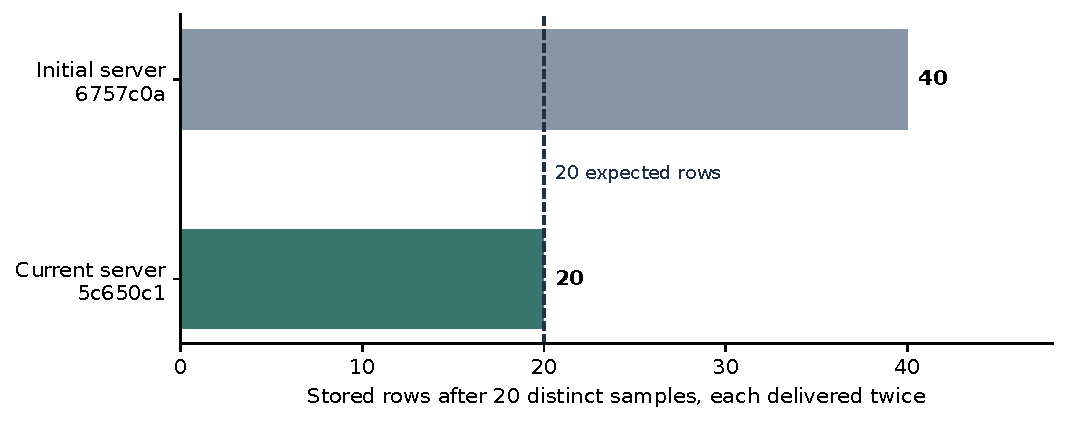
\includegraphics[width=.88\textwidth]{idempotency_improvement.pdf}
\caption{Measured chronological improvement in backend persistence. Forty successful responses represent twenty unique samples delivered twice. The baseline creates twenty extra rows; the current API preserves twenty unique records. The comparison excludes handset and network behaviour.}\label{fig:improvement}
\end{figure}

\subsection{Installation and execution procedure}
The release APK and source archive are distributed under \path{release/}. The recorded APK is version 1.0.0, code 13, minimum API 24 and target API 37. Its SHA-256 is \path{417c12efa634e960b5e3f0ab680a14951b4357a8580f59eb7b7c75caea206378}. Installation and launch on Samsung SM-S948B with Android 17 are recorded alongside 709 native interface checks. The following procedure documents replication of the separate account, server and interface paths. The operational guide is \path{docs/SERVER.md}.
\begin{enumerate}
\item Prepare the Python environment from \path{requirements.txt}; initialise the local server using \code{./carectl init --host YOUR_LAN_IP}. Keep generated keys private.
\item Use \code{./carectl start} and \code{./carectl status} to check HTTPS service readiness. Ensure the public CA bundled in the APK matches that server. Follow \path{docs/SERVER.md} when regenerating a build.
\item Install \path{release/CareMonitor-1.0.0.apk} using Android's authorised local installation flow and retain its hash and device identity. The recorded device uses Android 17/API 37; its interface tests do not grant permissions or activate sensors.
\item Use fictional adult and caregiver accounts for server experiments. Registration presents role, name, email and password as separate steps; the adult issues an invitation and approves the caregiver request. The server enforces that relationship.
\item Run \code{./carectl demo} with fictional adult credentials. This sends three synthetic rule samples; verify one episode and independent caregiver review. This command does not demonstrate a mobile model confidence view.
\item Exercise classification with fixed synthetic features through \path{/api/v1/ai/classify}; inspect the returned class, score and source. Reading persistence and retrieval use the separate readings endpoints. Care navigation and model inference have distinct presentation boundaries.
\item Reproduce the interface campaign with \path{mobile/scripts/test_onboarding_device.py}, selecting the exact device serial. The auxiliary instrumentation checks role selection, back navigation, password masking, enlarged registration forms and authenticated Settings using fictional in-memory profiles.
\end{enumerate}

\clearpage
\subsection{Scenario coverage matrix}
\small
\begin{longtable}{@{}P{24mm}P{62mm}P{67mm}@{}}
\caption{Reproducible scenarios, observed evidence and execution boundaries.}\\
\toprule Scenario & Input and expected result & Recorded evidence and scope\\\midrule\endfirsthead
\toprule Scenario & Input and expected result & Recorded evidence and scope\\\midrule\endhead
Normal & Fixed synthetic normal features; return Normal and score; valid normal snapshots create no rule episode & Model/API execution; classification is a server result, separate from care navigation\\
Deteriorating & Move from eligible normal snapshots to three distinct abnormal snapshots; one episode after persistence & Sustained condition and recovery test in isolated server fixtures\\
Critical & Select known Critical CSV fixture; return expected class; independently exercise an abnormal rule sequence & Held out model matrices and server episode campaign; delivery rate is a separate measure\\
Missing data & Omit required model feature; reject. Missing optical contact must not trigger or recover a rule & Missing feature and invalid contact tests; care views retain explicit unknown states\\
Invalid data & NaN, unexpected field, unsupported feature or stale age; reject classification & \path{test_ml.py}, \path{test_ai_api.py}, request limits tests\\
Network failure & Lose upload response and retry same ID; retain one row and active episode & Matched backend comparison and relay policies; excludes physical radio interruption\\
Unauthorised & Query unlinked adult, then revoke previously approved caregiver; disclose no resource & Server IDOR and revocation tests; native caregiver wearable controls are also rejected\\
Recovery & Three eligible observations no longer meeting the rule; recover episode; later new sustained event may create another & Sustained condition recovery test; review is not recovery\\\bottomrule
\end{longtable}
\normalsize

Exact automated anchors in \path{tests/test_api.py} include \path{test_sustained_condition_one_episode_valid_recovery_then_new_episode}, \path{test_idempotency_conflict_and_capture_order}, \path{test_idor_cannot_read_or_write_other_patients} and \path{test_revoke_removes_data_and_queued_notifications}. Model input boundaries are exercised by \path{tests/test_ai_api.py::test_synthetic_api_rejects_device_and_missing_features}. These names locate executable checks; they do not represent installed Android tests.

\subsection{Application latency and improvement protocol}
Select an initial revision and an improved revision before the experiment. Use the same device, dataset fixture IDs, server hardware, network and permissions. After identical warmup, record at least thirty trials per scenario. Measure API time from dispatch to parsed response, and caregiver latency from the first qualifying synthetic input to visible notification. Keep raw timestamps, request IDs, failed trials and timeouts. Report N, mean, p50 and p95 for both revisions; do not silently omit failed deliveries.

For missed Critical alerts, divide Critical scenarios without a required visible alert within the declared observation window by all Critical scenarios that should generate one. For false Warnings, divide Normal scenarios producing an unwanted Warning by all Normal scenarios. Define the observation window before testing. Model predictions and rule alerts have different semantics; a latency experiment must identify the rule output and its observation window. Separately report duplicates and data loss after reconnection.
\FloatBarrier
\clearpage
\section{Historical development images}
\label{app:images}
The following supplied captures are cropped for relevance. No output or values have been synthesised. Source paths and crop coordinates are recorded in \path{evidence/crop_manifest.json}. They document historical software experiments, separately from the assembly in Figure~\ref{fig:hardware-photo} and the Android code 13 interface campaign.

\begin{figure}[htbp]\centering
\begin{subfigure}{.485\textwidth}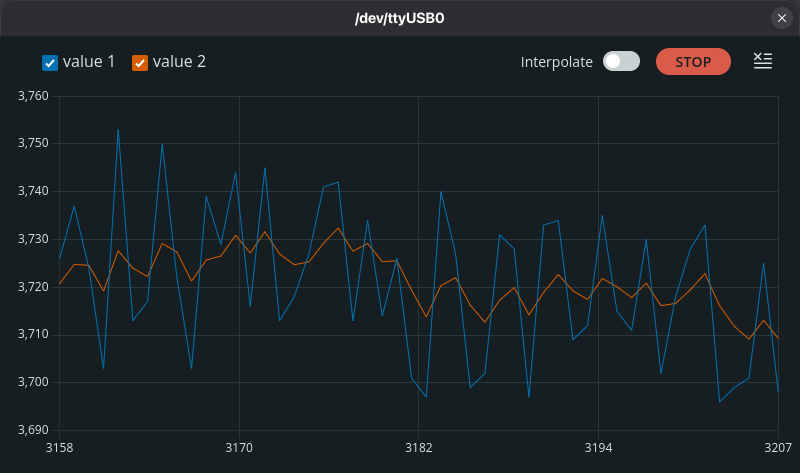
\includegraphics[width=\linewidth]{adc_smoothing.png}\caption{Raw and smoothed ADC traces.}\end{subfigure}\hfill
\begin{subfigure}{.485\textwidth}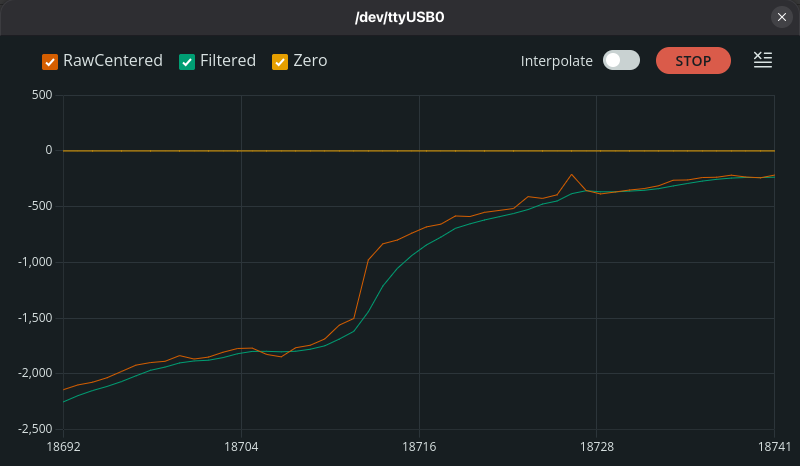
\includegraphics[width=\linewidth]{centered_filter.png}\caption{Centred input, filtered output and zero reference.}\end{subfigure}
\caption{Serial plotting during development on 13 October 2026. The uncalibrated ADC plots support qualitative signal conditioning observations. Axes do not establish physical time, clinical accuracy or a quantified before and after noise reduction.}\label{fig:adc}
\end{figure}

\begin{figure}[htbp]\centering
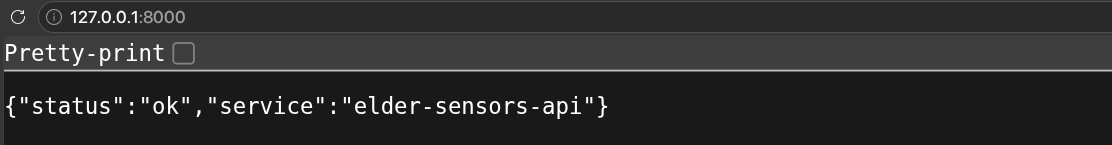
\includegraphics[width=\textwidth]{api_health.png}
\vspace{5mm}
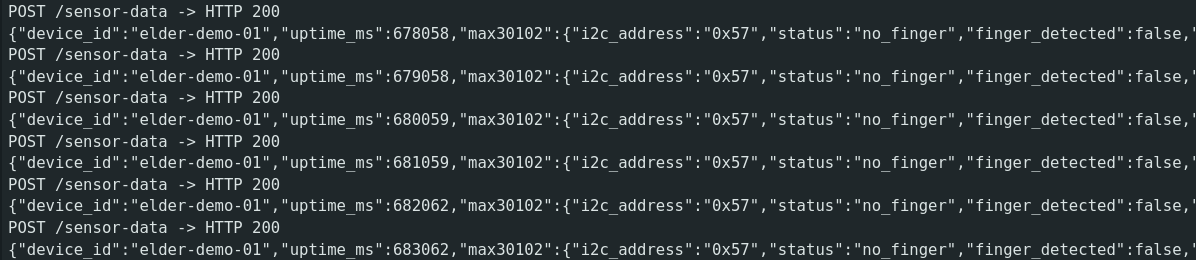
\includegraphics[width=\textwidth]{post_200_no_finger.png}
\caption{Local API availability and successful historical uploads on 13 October 2026. The old \code{/sensor-data} route returns HTTP 200 while the optical module reports \code{no_finger}. Successful transport does not establish measurement validity, persistent storage or the final versioned API.}\label{fig:http-history}
\end{figure}

\begin{figure}[htbp]\centering
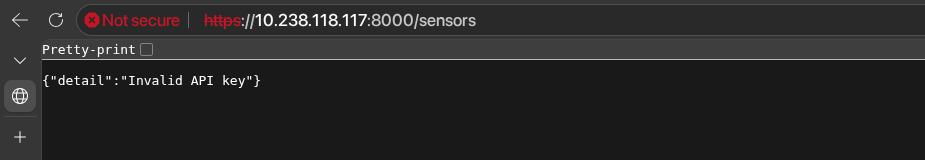
\includegraphics[width=\textwidth]{api_rejection.png}
\caption{Historical authentication rejection on 15 October 2026. The browser reports an invalid API key and also marks the connection insecure. This establishes a negative authentication path for that version; it is not evidence of trusted HTTPS or the current account based contract.}\label{fig:auth-history}
\end{figure}
\FloatBarrier
\clearpage
\section{Project team and development history}
\label{app:contribution}
The team roster identifies the academic submission. Repository chronology provides the technical change record; commit metadata is not used to infer a division of personal responsibilities or an individual contribution multiplier.

\begin{tabularx}{\textwidth}{@{}Y P{35mm}@{}}\toprule
Team member & Student ID\\\midrule
Nathan Ratichon & 2362789\\
Guannan Ge & 2364229\\
Jose Manuel Cortes Ceron & 2686162\\
Cheng Zhang & 2361292\\\bottomrule
\end{tabularx}

The tutor is Matilda Isaac. The names and IDs are reproduced as supplied by the team and are maintained in \path{metadata.tex}.

\begin{tabularx}{\textwidth}{@{}P{22mm}P{26mm}Y@{}}\toprule
Date & Commit & Recorded subject\\\midrule
25 Oct 2026 & \texttt{27a72d4} & Initial commit\\
25 Oct 2026 & \texttt{6757c0a} & upload files\\
25 Oct 2026 & \texttt{7e6c494} & upload csv files and data for ML part\\
26 Oct 2026 & \texttt{5c650c1} & update: mayor fixes\\\bottomrule
\end{tabularx}

The recorded Git identity is Jos\'e Manuel Cortes Cer\'on. The four commits establish the baseline chronology. The Android interface campaign and this report revision also include local working-tree changes, identified by the release input hashes rather than represented as additional commits. This preserves the distinction between committed history, supplied documentation and the exact built artefact.

\clearpage
\section{Demonstration protocol and evaluation boundaries}
\label{app:acceptance}
The demonstration separates three observable layers: native care navigation, synthetic server evaluation and the physical bench assembly. This structure prevents a successful result in one layer from being used as evidence for a different layer.

\begin{enumerate}
\item Identify APK 1.0.0/code 13 and its hash. Open the application on the Samsung and show the four-step account setup, explicit role selection, password visibility control and fixed primary action. The 709-check campaign records these interface behaviours, including registration text at 200\%.
\item Show role-specific navigation and grouped Settings. The caregiver has no wearable connection control; the connection page is inside authenticated Settings. The adult's source-defined wearable guide separates preparation, pairing, selection and recent-sample verification.
\item Run fixed Normal, Warning and Critical fixtures through the authenticated classification API. Display the response class, model score and synthetic source separately from the care interface. Readings and rule episodes use their own storage endpoints.
\item Exercise a sustained rule condition with three eligible samples, inspect the stored episode and compare the two caregivers' private inboxes. The recorded HTTPS fixture establishes fanout and independent review at the server boundary.
\item Retry a sample after a lost response and compare its stored identity. Show invalid or missing inputs producing rejection or an unknown state. The backend comparison and policy tests establish these properties without assigning handset delivery latency to them.
\item Present the physical assembly in Figure~\ref{fig:hardware-photo}, the source architecture and the recorded diagnostic aggregate. Explain which result comes from an image, a serial observation, a server test or a native interface check.
\end{enumerate}

\begin{table}[H]\small
\caption{Evaluation domains and the evidence supporting each claim.}\label{tab:acceptance}
\begin{tabularx}{\textwidth}{@{}P{34mm}Y P{37mm}@{}}\toprule
Domain & Recorded evidence and interpretation & Assessment relationship\\\midrule
Android interface & Installed code 13; 709 native checks; registration at text scale 2.0; role and Settings navigation & Mobile functionality and programming\\
Classification & Two trained models, held out matrices and authenticated server inference; scores describe synthetic classes & AI and REST\\
Persistence and alerts & 88 Python tests, 17 loopback HTTPS checks, 20 matched retry pairs and 20 episode trials & Data integration and testing\\
Hardware assembly & Original team photograph and 25-message diagnostic aggregate; image and runtime observation have distinct scope & Architecture and demonstration\\
Development trace & Team roster, four baseline commits and input hashes for the local release & Configuration and documentation\\\bottomrule
\end{tabularx}
\end{table}

The care Activity presents readings, alerts and settings; the history endpoint and chart component are separate from its current navigation, and classification scores are exposed by the server interface. The measured results concern these explicit system boundaries. They establish neither clinical efficacy nor a medical safety certification, and they do not turn a synthetic class score into a disease probability.
